\section{Introduction}
In the homework, a classification model of heat sensors on train axes is made. Data have been furnished, containing samples of each sensor and the opinion of expert saying if it was a false alarm or if the train as a real problem for multiple train passage. The work have been split in 3 parts, features engineering, features selection and classification. 

\vspace{-10mm}

\section{Data set}
Two data sets have been provided, one for training and one for validation, which will only be used for validation. Table \ref{tab:Look} shows the distribution of the samples state. It has to be noted that in further application only the long identification has been used. If the classification using the long identification were leading to many wrong short classification, a two step classification could be consider. 

\createtable[h]
{Title1} 
{Data sets outlook}
{\label{tab:Look}} 
{\begin{tabular}{l|c|c|}
& Training & Validation \\\hline
F & 592 & 146 \\
E & 69 & 17 \\
Z & 47 & 11 \\
\end{tabular}}
{}

\section{Features engineering}
In this section different features are selected by detector, i.e. for example the mean for 8 detectors, and by side. It has be done like this to allow the machine learning algorithm to look for some classification factors for each detectors but also per side.

The following features have been selected. 

\begin{itemize}
    \item Mean
    \item Variance
    \item Skewness
    \item Kurtosis
    \item Crest factor
\end{itemize}

This choice has been done while looking into the data. Indeed, the most common case is FHA and seems to have a pattern. As shown in figure \ref{fig:samples}, one side have a really low mean while the other have a high mean and really low variance. Selecting mean, variance and crest factor was therefore making sens. The Kurtosis might allow to detect healthy sample that should follow a similar shape as the right-hand side with a higher variance. If bad performance other features could been added later.

\createfigure[H]
  {}
    {Sample example}
    {\label{fig:samples}}
    {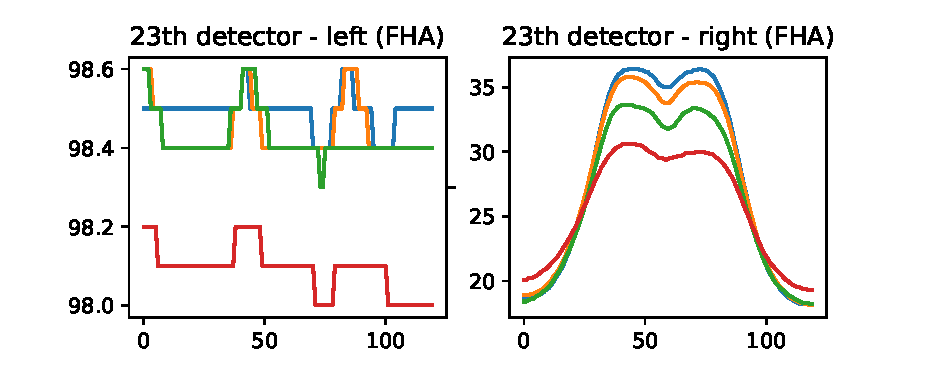
\includegraphics[width = \textwidth]{figures/sample.eps}}
    {}

\section{Features engineering}
The combination of the 5 features for every detectors and the 2 sides give a total of 50 features. To avoid a too high computation time on redundant features some of them are going to be selected. To select them a wrapper methods is going to be used with the selected classification algorithm, a random forest classifier. 

Before selecting the features the training set is going to be divided into 5 equals part, 4 of them are going to be used as training and 1 for testing. Then another one is used as testing etc. .

According to the size of the data set, the training of the model should not be too long, so rather high number of features can be selected. That is way a backward model has been preferred. The same argument apply for the choice of a wrapper methods rather than a filter approach. 

For the selection of feature a backward selection is performed, using trying to maximise the following.

  $f(Y)=\frac{1}{N} \sum_{k=1}^{N} W_{k},$ where $W_{k}\left\{\begin{array}{c}1 \text { if sample } Y_{k} \text { bewertung is correct } \\ 0.7 \text { if sample } Y_{k} \text { 'kurzbewertung is correct } \\ 0 \text { otherwise }\end{array}\right.$
  
In figure \ref{fig:Nfeature} features are selected, the relation between time of execution, performance and number of selected features is shown. It was expected that performance would have decrease with a lower number of features but it did not. An explanation could be the over-representation of some features having the same cause.

Same with the training time. But as the training time is rather low the time it took depend on the availability of power of the computer and might be bias. 
As the ratio performance/ time seems to be the best around 15 features, 15 are going to be selected, so a backward selection might not have been the best choice after all. 



\createfigure[h]
  {}
    {Selection of features}
    {\label{fig:Nfeature}}
    {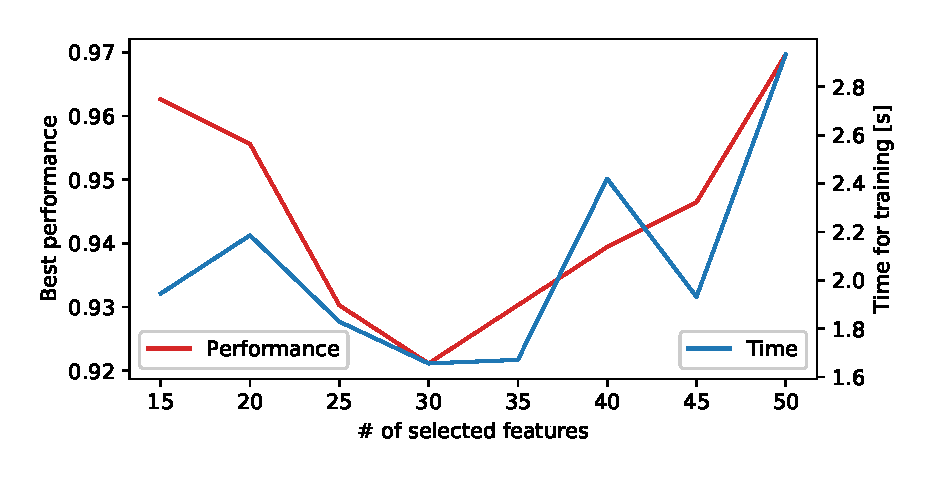
\includegraphics[width = 0.9\textwidth]{figures/Nfeature.eps}}
    {}


Then a random forest model is design with the selected features. Then the performance of the model is compute as the value of the function with predicted and actual value of the test data set.

\section{Classification}
The same random forest algorithm is used. It is trained with the best performing train data set. The random forest has been chosen as it is better than a normal tree, has low risk of over fitting and allow the full usage of the computation power ( easy implementation of parallel computing ).


\section{Results}
\createtable[h]
{Title1} 
{Results}
{\label{tab:Results}} 
{\begin{tabular}{|c|l|c|c|c|c|c|c|c|c|c|c|c|}
\cline{3-13}
\multicolumn{2}{c|}{\multirow{2}{*}{}} &\multicolumn{11}{c|}{Predicted}\\ \cline{3-13}
\multicolumn{2}{c|}{} & E & F & Z & ZD & EH & EHWB & FHA & FHF & FHR & FHRB & FHRD\\\hline
\multirow{11}{*}{\begin{sideways}Real\end{sideways}} & E & 16 & 1 & 0 & 0 & 0 & 0 & 0 & 0 & 0 & 0 & 0\\  \cline{2-13}
& F & 0 & 142 & 4 & 0 & 0 & 0 & 0 & 0 & 0 & 0 & 0\\  \cline{2-13}
& Z & 2 & 0 & 9 & 0 & 0 & 0 & 0 & 0 & 0 & 0 & 0\\  \cline{2-13}
& ZD & 0 & 0 & 0 & 9 & 0 & 2 & 0 & 0 & 0 & 0 & 0\\  \cline{2-13}
& EH & 0 & 0 & 0 & 0 & 0 & 0 & 0 & 1 & 0 & 0 & 0\\ \cline{2-13}
& EHWB & 0 & 0 & 0 & 0 & 0 & 16 & 0 & 0 & 0 & 0 & 0\\\cline{2-13}
& FHA & 0 & 0 & 0 & 0 & 0 & 0 & 135 & 0 & 0 & 0 & 0\\\cline{2-13}
& FHF & 0 & 0 & 0 & 2 & 0 & 0 & 0 & 2 & 0 & 0 & 0\\  \cline{2-13}
& FHR & 0 & 0 & 0 & 1 & 0 & 0 & 0 & 0 & 0 & 0 & 0\\  \cline{2-13}
& FHRB & 0 & 0 & 0 & 1 & 0 & 0 & 0 & 0 & 0 & 0 & 0\\ \cline{2-13}
& FHRD & 0 & 0 & 0 & 0 & 0 & 0 & 0 & 0 & 0 & 0 & 5\\ \hline
\end{tabular}}
{}


\section{Conclusion} 

As the table \ref{tab:Results} show, there is really few miss classifications on short bewertung. As it is rather low, a two step classification (short than long) is not needed. The results are pretty good, maybe too much. The algorithm have a performance of 0.96, which is really good. There is some miss classification but mainly with 'Z' type, one could assume that 'Z' type will still be analysed in the future by expert. Concerning long bewertung the FHA which is the most represented category has not been miss classified. An explanation could be that as it is the most represented ( by far), they have been way more training to detect this type. Where the other have been more miss classified, the opposite argument apply. As they are under represented it is difficult for the algorithm to really determine a pattern. 

